\begin{savequote}[45mm]
The new star in Cygnus that I first observed on August 8, 1600, was initially of third magnitude. I determined its position by measuring its distance from Vega and Albireo.
\qauthor{Willem Janszoon Blaeu}
\end{savequote}

\chapter{Introduction}

\section{P Cygni Stars}

P Cygni (or 34 Cygni) is a luminous blue variable star (LBV) that has been studied extensively \cite{1953PDAO....9....1B, hutchings1969expanding, elliott20225, underhill1966supergiants,mizumoto2018newly}. Willem Janszoon Blaeu, a Dutch cartographer and student of the astronomer Tycho Brahe is considered to have provided the first known set of observations of 34 Cygni in the year 1600 \cite{deGrootPCygni}. The stellar spectrum of 34 Cygni is peculiar. It exhibits the characteristics of a B type supergiant except that almost all absorption lines are blue shifted with a red shifted emission component \cite{hutchings1969expanding}. This characteristic line profile can be clearly observed in proximity to the H$\alpha$ line which is placed at \textasciitilde 6563\r{A} \cite{zhang2021catalog,traven2015gaia}

P Cygni type stars or simply, \emph{P Cygni stars} are stars that exhibit line profiles that are similar to the characteristic profile of 34 Cygni. The spectra of these stars show characteristic absorption, emission and wide absorption sub-components \cite{zhang2021catalog}. The red shifted counterpart to the P Cygni stars have also been observed. These now belong to a class of objects known as the Inverted P Cygni stars or \emph{Inverse P Cygni stars}. 

\begin{figure}[t]
\centering
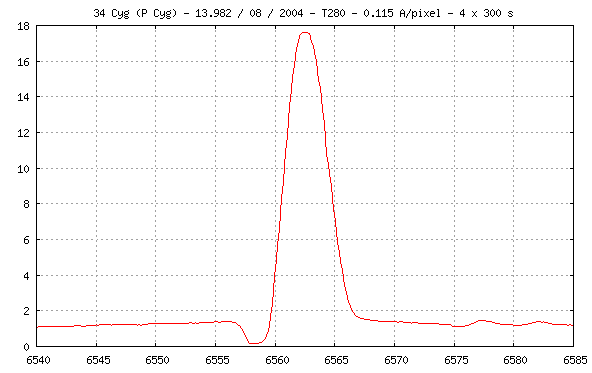
\includegraphics[scale=.40]{figures/34cygni.png}
\caption{The normalised spectrum of 34 Cygni around H$\alpha$.}
\end{figure}

It is hypothesised that distinct physical processes within these stars generate the respective line profiles \cite{hou2016catalog}. Beals was the first to demonstrate that P Cygni and Inverse P Cygni line profiles can be explained by the interaction between the stellar disk of a hot, massive young star and the expanding or contracting shell of gas surrounding the star \cite{1953PDAO....9....1B}. 

\begin{figure}[h]
\centering
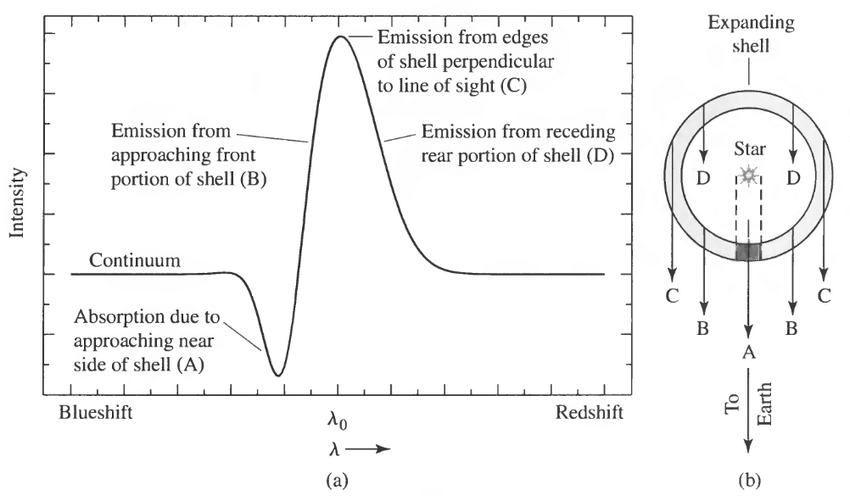
\includegraphics[scale=.40]{figures/expandingpcygni.png}
\caption{Cartoon depicting the physical mechanism by which a P Cygni line profile is generated. Reproduced from Kasai (2013)\cite{kasai2013type}}
\end{figure}

\section{Historical Perspective}

One of the first modern attempts at identifying and characterising P Cygni stars was by Beals (1953) \cite{1953PDAO....9....1B}. This work identified all the known Northern Hemisphere observations of P Cygni stars into a comprehensive catalog based on spectral profiles. This catalog was compiled by examining spectra using the naked eye between the years 1928 and 1946. The catalog was then used to generate hypotheses of how P Cygni stars may exchange material with their surroundings via accretions, inflows and outflows. The morphological properties of the spectra were then used to calculate the wind velocities of inflows and outflows. The work also presents an early attempt at classification of P Cygni stars based on their morphology. The characteristic P Cygni and inverted P Cygni profiles are included as distinct classes.



